\let\negmedspace\undefined
\let\negthickspace\undefined
\documentclass[journal,12pt,twocolumn]{IEEEtran}
\usepackage{cite}
\usepackage{amsmath,amssymb,amsfonts,amsthm}
\usepackage{algorithmic}
\usepackage{graphicx}
\usepackage{textcomp}
\usepackage{xcolor}
\usepackage{txfonts}
\usepackage{listings}
\usepackage{enumitem}
\usepackage{mathtools}
\usepackage{gensymb}
\usepackage{comment}
\usepackage[breaklinks=true]{hyperref}
\usepackage{tkz-euclide} 
\usepackage{listings}
\usepackage{gvv}                                        
\def\inputGnumericTable{}                                 
\usepackage[latin1]{inputenc}                                
\usepackage{color}                                            
\usepackage{array}                                            
\usepackage{longtable}                                       
\usepackage{calc}                                             
\usepackage{multirow}                                         
\usepackage{hhline}                                           
\usepackage{ifthen}                                           
\usepackage{lscape}
\newtheorem{theorem}{Theorem}[section]
\newtheorem{problem}{Problem}
\newtheorem{proposition}{Proposition}[section]
\newtheorem{lemma}{Lemma}[section]
\newtheorem{corollary}[theorem]{Corollary}
\newtheorem{example}{Example}[section]
\newtheorem{definition}[problem]{Definition}
\newcommand{\BEQA}{\begin{eqnarray}}
\newcommand{\EEQA}{\end{eqnarray}}
\newcommand{\define}{\stackrel{\triangle}{=}}
\theoremstyle{remark}
\newtheorem{rem}{Remark}
\begin{document}
\bibliographystyle{IEEEtran}
\vspace{3cm}
\title{NCERT 11.9.2 16Q}
\author{EE23BTECH11021 - GANNE GOPI CHANDU$^{*}$% <-this % stops a space
}
\maketitle
\newpage
\bigskip
\renewcommand{\thefigure}{\theenumi}
\renewcommand{\thetable}{\theenumi}
\bibliographystyle{IEEEtran}
\textbf{Question}\\
Between 1 and 31, m numbers have been inserted in such a way that the resulting sequence is an A.P. and 
the ratio of 7
th and (m - 1)
th numbers is 5:9. Find the value of m.\\
\textbf{Solution}\\
\begin{table}[!h]
\begin{center}
\renewcommand\thetable{1}
\begin{tabular}{ |c|c|c| } 
  \hline
    Symbol & Value & description \\ 
  \hline
  $x(0)$ & 1 & First term of A.P  \\ 
  \hline
  x(n) & 31 & last term \\
  \hline
  d & 2 & Common difference \\ 
  \hline
  n & m+2 & number of terms \\
  \hline
  m & 14 & number of terms inserted \\
  \hline
\end{tabular}
\end{center}
\caption{}
\end{table}\\
The last term is
\begin{align}
x(n)&=x(0)+nd\\
31 &= 1 + \brak{m + 1}d \\
30 &= \brak{m + 1}d \\
\frac{30}{m + 1} &= d \label{eq11.9.2.4}
\end{align}
Now $7$th and $\brak{m-1}$th terms
\begin{align}
\implies x\brak{7} &= x(0) + 7d\label{eq11.9.2.5}\\
\implies x\brak{m-1} &= x(0) + \brak{m-1}d\label{eq11.9.2.6}
\end{align}
Given 
\begin{align}
\frac{x\brak{7}}{x\brak{m-1}} = \frac{5}{9} \label{eq11.9.2.7}
\end{align}
From  equations \eqref{eq11.9.2.5} and \eqref{eq11.9.2.6} the augmented matrix is:\\
\begin{align}
 \myvec{
   1 & 7 & x\brak{7}
   \\
   1 & m-1 & x\brak{m-1}
 }
 \xleftrightarrow[]{R_2 \leftarrow {R_2-R_1}}
 \myvec{
   1 & 7 & x\brak{7}
   \\
   0 & m-8 & x\brak{m-1}-x_7
 }
 \\
 \xleftrightarrow[]{R_2 \leftarrow {\frac{1}{m-8}R_2}}
 \myvec{
   1 & 7 & x\brak{7}
   \\
   0 & 1 & \frac{x\brak{m-1}-x_7}{m-8}
 }
 \\
 \xleftrightarrow[]{R_1 \leftarrow {R_1-7{R_2}}}
 \myvec{
   1 & 0 & x_7-7\brak{\frac{x\brak{m-1}-x\brak{7}}{m-8}}
   \\
   0 & 1 & \frac{x\brak{m-1}-x\brak{7}}{m-8}
 }
 \\
 \implies \myvec{
   x\brak{0}
   \\
   d
 }
 =
 \myvec{
   x_7-7\brak{\frac{x\brak{m-1}-x\brak{7}}{m-8}}
   \\
   \frac{x\brak{m-1}-x\brak{7}}{m-8}
 }
\end{align}
part 1\\
from equation \eqref{eq11.9.2.7}\\
\begin{align}
    x\brak{0}&=x\brak{7}-7\brak{\frac{x\brak{m-1}-x\brak{7}}{m-8}}\\
    1&=x\brak{7}-7\brak{\frac{x\brak{m-1}-x\brak{7}}{m-8}}\\
    1&=x\brak{7}-7\brak{\frac{x\brak{7}\brak{\frac{9}{5}}-x\brak{7}}{m-8}}\\
    1&=x\brak{7}\brak{\brak{m-8}-\frac{28}{5}}
\end{align}
part 2\\
from equations \eqref{eq11.9.2.4} and \eqref{eq11.9.2.7}\\
 \begin{align}
    d&=\frac{x\brak{m-1}-x\brak{7}}{m-8}\\
    \frac{30}{m+1}&=\frac{x\brak{7}\brak{\frac{4}{9}}}{m-8}\\ \label{eq11.9.2.18}
    x\brak{7}&=\frac{75\brak{m-8}}{2\brak{m+1}}
 \end{align}
Substituting \eqref{eq11.9.2.18} in part 1\\
 \begin{align}
    m-8&=\frac{75\brak{m-8}\brak{5m-68}}{10\brak{m+1}}\\
    2\brak{m+1}&=15\brak{5m-68}\\
    2m+2&=75m-1020\\
    73m&=1022\\
    m&=14
 \end{align}
General term of AP as 
\begin{align}
    x\brak{n}=\brak{2n-1}u(n)
\end{align}
\begin{figure}[!h]
    \centering
    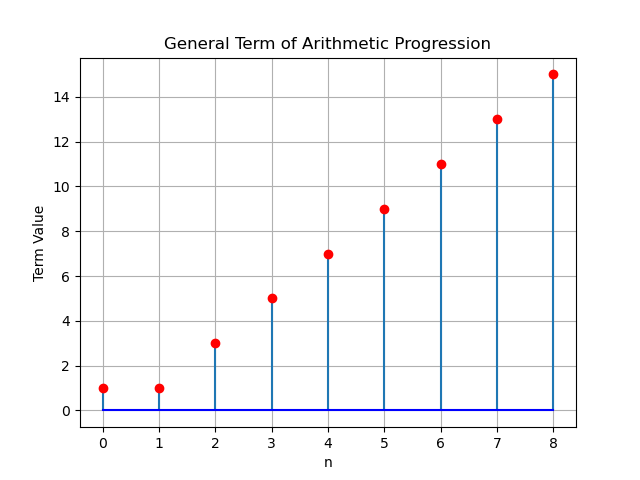
\includegraphics[width=1.0\linewidth]{test.png}
    \caption{Plot of x(n) vs n}
    \label{fig:1}
\end{figure}\\
The Z-Transform Equation for x\brak{n} is\\
\begin{align}
    X\brak{z}&=\sum_{n=-\infty}^{\infty}\brak{2n-1}z^{-n}u\brak{n} \\ \implies X\brak{z}&=\sum_{n=\infty}^{\infty}\brak{2n}z^{-n}u\brak{n} -\sum_{n=-\infty}^{n=\infty}z^{-n}u\brak{n}\\
   \implies X(z)&=2\sum_{n=0}^{\infty}\dfrac{n}{z^{n}}-U\brak{z}
\end{align}
\text{The first part of summation is}\\
\begin{align}
   \implies S\brak{\infty}&=\dfrac{z^2}{\brak{z-1}^{2}}
\end{align}
\text{The second part of summation is}\\
\begin{align}
   U\brak{z}=\dfrac{1}{1-z^{-1}}
\end{align}
The result is,
\begin{align}
    X\brak{z}&=2S_\infty-U\brak{z}\\
    X\brak{z}&=\dfrac{z^2}{\brak{z-1}^{2}}-\dfrac{1}{1-z^{-1}}\\
    X\brak{z}&=\dfrac{z^2+z}{\brak{z-1}^{2}}
\end{align}
(ROC) \(|z| > 1\).\\
\end{document}
